In this section, we demonstrate that the interpolation points can also be
selected from a Voronoi tessellation procedure. For a $d$\hyp{}dimensional
space, the Voronoi tessellation partitions a set of points $\{r_{i}\}_{i=1}^{N_
{g}}\subset\BBR^{d}$ into a number of disjoint cells. The partition is based on
the distance of each point to a finite set of points, called its generators. In
our context, let $\{\rhat_\mu\}_{\mu=1}^{N_{\mu}}$ denote such a set of
generators, and the corresponding cell, $\calC_\mu$, of a given generator
$\rhat_\mu$ is defined as a cluster of points
\begin{equation}\label{eqn:vcell}
  \calC_\mu = \{r_{i} ~\vert~\dist(r_{i}\,,\, \rhat_\mu) <
  \dist(r_{i}\, ,\, \rhat_\nu) \textrm{ for all } \nu \neq \mu\}\,.
\end{equation}
The distance can be chosen to be any metric, e.g. the $L_2$ distance as $\dist
(r\,,\,r')=\norm{r-r'}_2$. In the case when the distances of a point $r$ to
$\rhat_\mu, \rhat_\nu$ are exactly the same, we may arbitrarily assign $r$ to
one of the clusters.

The \emph{centroidal Voronoi tessellation} (CVT) is a specific type of Voronoi
tessellation in which the generator $\rhat_\mu$ is chosen to be the centroid of
its cell. Given a weight function $\rho(r)$ (such as the electron density), the
centroid of a cluster $\calC_\mu$ is defined as
\begin{equation}\label{eqn:centcomp}
  c(\calC_\mu) = \frac{\sum_{r_{j}\in \calC_\mu} r_j\;\rho(r_j)}{\sum_{r_j\in
  \calC_\mu}\rho(r_j)}\,.
\end{equation}
Combined with the $L_2$\hyp{}distance, CVT can be viewed as a minimization
problem over both all possible partition of the cells and the centroids as 
\cite{MacQueen1967}
\begin{equation}\label{eqn:CVT}
  \{\calC_\mu^\ast,c_{\mu}^{*}\} = \argmin_{\{\calC_\mu, \Bc_{\mu}\}} \sum_
  {\mu=1}^{N_{\mu}} \sum_{r_k\in \calC_\mu}\rho(r_k)\norm{r_i-c_{\mu}}^2\,,
\end{equation}
and the interpolation points are then chosen to be the minimizers
$\rhat_\mu=c_{\mu}(\calC_\mu^\ast)=c_{\mu}^{\ast}$. Following the discussion in
\cref{cvtsec:int}, the electron density as the weight function~\eqref{eqn:CVT}
enforces that the interpolation points should locate at points where the
electron density is significant and hence satisfies the requirement (1). Since
the cells $\calC_\mu^\ast$ are disjoint, the centroids $c_{\mu}^\ast$ are also
separated by a finite distance away from each other and hence satisfies the
requirement (2). Because the ISDF decomposition is a highly nonlinear process,
in general we cannot expect the choice of interpolation points from CVT
decomposition to maximally reduce the error of the decomposition. Instead, we
demonstrate that the choice of the interpolation points from CVT approximately
minimizes the residual for the ISDF decomposition, and hence provides a
heuristic solution to the problem of finding interpolation points.

\begin{theorem}
  When the set of electron orbitals $\{\varphi_i\}$ are Lipschitz continuous,
  CVT method approximately minimizes the residual error of the ISDF
  decomposition.
\end{theorem}
\begin{proof}
  For simplicity we assume the limiting case where $\varphi_{i}=\psi_{i}$, and
  hence each row of $Z$ is $Z(r)=[\varphi_{i}(r)\varphi_{j}(r)]_{i,j=1}^N$.

  Now suppose we cluster all matrix rows of $Z$ into sub\hyp{}collections $
  \{\calC_\mu\}_{\mu=1}^{N_\mu}$, and for each $\calC_\mu$ we choose a
  representative matrix row $Z(r_\mu)$. Then the error of the ISDF can be
  approximately characterized as
  \begin{equation}\label{eqn:ISDFerror}
    R = \sum_{\mu = 1}^{N_\mu}\sum_{r_k\In \calC_\mu}\norm{Z(r_k)- \Proj_{\Span
    \{Z(r_{\mu})\}}Z(r_k)}^2,
  \end{equation}
  where the projection is defined according to the $L_2$ inner product as
  \begin{equation}\label{eqn:Zprojection}
    \Proj_{\Span\{Z(r_{\mu})\}}Z(r_k) = \frac{Z(r_{k})\cdot Z(r_\mu)}{Z
    (r_\mu)\cdot Z(r_\mu)}Z(r_{\mu}).
  \end{equation}
  Let $\Phi$ be the $N_{g} \times N$ matrix with each row $\Phi(r) = 
  [\varphi_i(r)]_{i=1}^N$, then the electron density $\rho(r)$ is equal to
  $\Phi(r)\cdot \Phi(r)$. Using the relation
  \begin{equation}\label{eqn:ZtoPhi}
    Z(r_\mu)\cdot Z(r_\mu) = (\Phi(r_{\mu})\cdot \Phi(r_{\mu}))^2 = \rho(r_
    {\mu})^2,
  \end{equation}
  we have
  \begin{align}
    R &= \sum_{\mu=1}^{N_\mu}\sum_{r_k\In \calC_\mu}\rho(r_k)^2 \left(1-
    \frac{(\Phi(r_{k})\cdot\Phi(r_{\mu}))^4}{\rho(r_k)^2\rho(r_\mu)^2}\right)\\
    &= \sum_{\mu=1}^{N_\mu}\sum_{r_k\in \calC_\mu}\rho(r_k)^2 [1-\cos^4(\theta
    (r_k,r_\mu))]\,.
  \end{align}
  Here $\theta(r_{k},r_{\mu})$ is the angle between the vectors $\Phi(r_{k})$
  and $\Phi(r_{\mu})$. Since
  \begin{align}
    \rho(r_k) [1-\cos^4(\theta(r_k,r_\mu))] &\Leq 2 \Phi(r_{k})\cdot \Phi(r_
    {k})\sin^{2}(\theta(r_k,r_\mu)) \\
    &\Leq 2 \norm{\Phi(r_{k})-\Phi(r_{\mu})}^2,
  \end{align}
  we have
  \begin{align}
    R &\Leq 2 \sum_{\mu=1}^{N_\mu}\sum_{r_k\in \calC_\mu}\rho(r_k) 
    \norm{\Phi(r_{k})-\Phi(r_{\mu})}^2 \\
    &\approx 2 \sum_{\mu=1}^{N_\mu}\sum_{r_k\in \calC_\mu}\rho(r_k)
    \norm{\nabla_{r}\Phi(r_{\mu})}^2 \norm{r_{k}-r_{\mu}}^2.
  \end{align}
  If we bound the gradient of $\Phi(r)$ by its Lipschitz constant, or simply
  neglect the spatial inhomogeneity in the electron orbitals, we arrive at the
  minimization criterion for the centroidal Voronoi tessellation decomposition.
\end{proof}

Many algorithms have been developed to efficiently compute the Voronoi
tessellation \cite{medvedev1986algorithm}. One most widely used method is the
Llyod's algorithm \cite{lloyd1982least}, which in discrete case is equivalent to
the K\hyp{}Means algorithm \cite{MacQueen1967}. The K\hyp{}Means algorithm is an
iterative method that greedily minimizes the objective by taking alternating
steps between $\{\calC_\mu\}$ and $\{c_\mu\}$. In this work, we adopt a weighted
version of the K\hyp{}Means algorithm, which is demonstrated in 
\cref{alg:wkmean}. Note that the K\hyp{}Means algorithm can be straightforwardly
parallelized. We distribute the grid points evenly at the beginning. The
classification step is the most time consuming step, and can be locally computed
for each group of grid points. After this step, the weighted sum and total
weight of all clusters can be reduced from and broadcast to all processors for
the next iteration.


\begin{algorithm}
  \caption{Weighted K\hyp{}Means Algorithm to Find Interpolation Points for
  Density Fitting}\label{alg:wkmean}
  \SetKwInOut{Input}{Input}
  \SetKwInOut{Output}{Output}
  \SetKwRepeat{Do}{do}{while}
  \SetKwFor{For}{for}{}{end for}
  \SetKwIF{If}{ElseIf}{Else}{if}{}{else if}{else}{end if}
  \DontPrintSemicolon
  \Input{Grid points $\{r_i\}_{i=1}^{N_{g}}$, Weight function $\rho(r)$,
  Initial centroids $\{c^{(0)}_\mu\}$}
  \Output{Interpolation points $\{\rhat_\mu\}_{\mu=1}^{N_{\mu}}$}
  \textbf{Set} $t\gets 0$\;

  \Do{$\{c^{(t)}_\mu\}$ \textrm{\upshape not converged and maximum steps not
  reached}}{
    \textbf{Classification step:}\;
    \For{$i = 1$ \KwTo $N_g$}{
      Assign point $r_{i}$ to the cluster $\calC^{(t)}_{\mu}$
      \textbf{if} $c^{(t)}_\mu$ is the closest centroid to $r_i$\;
    }
    \;
    \textbf{Update step:}\;
    \For{$\mu = 1$ \KwTo $N_\mu$}{
      $c^{(t+1)}_\mu \gets
      {\sum_{r_{j}\in \calC^{(t)}_{\mu}}r_j\;\rho(r_j)}/{\sum_{r_j\in
      \calC^{(t)}_\mu}\rho(r_j)}$\;
    }
    \textbf{Set} $t\gets t+1$\;
  }
  \For{$\mu = 1$ \KwTo $N_\mu$}{
    \textbf{Set} $\rhat_\mu\gets c^{(t)}_{\mu}$\;
  }
\end{algorithm}

In order to demonstrate the CVT procedure, we consider the weight function $\rho
(r)$ given by the summation of four Gaussian functions in a 2D domain. The
initial choice of centroids, given by 40 uniformly distributed random points,
together with its associated Voronoi tessellation are plotted in \cref{fig:CVT} 
(a). \cref{fig:CVT} (b) demonstrates the converged centroids
and the associated Voronoi tessellation using the weighted K\hyp{}Means
algorithm. We observe that the centroids concentrate on where the weight
function is significant, and are well\hyp{}separated.

\begin{figure}[htbp]
  \begin{center}
    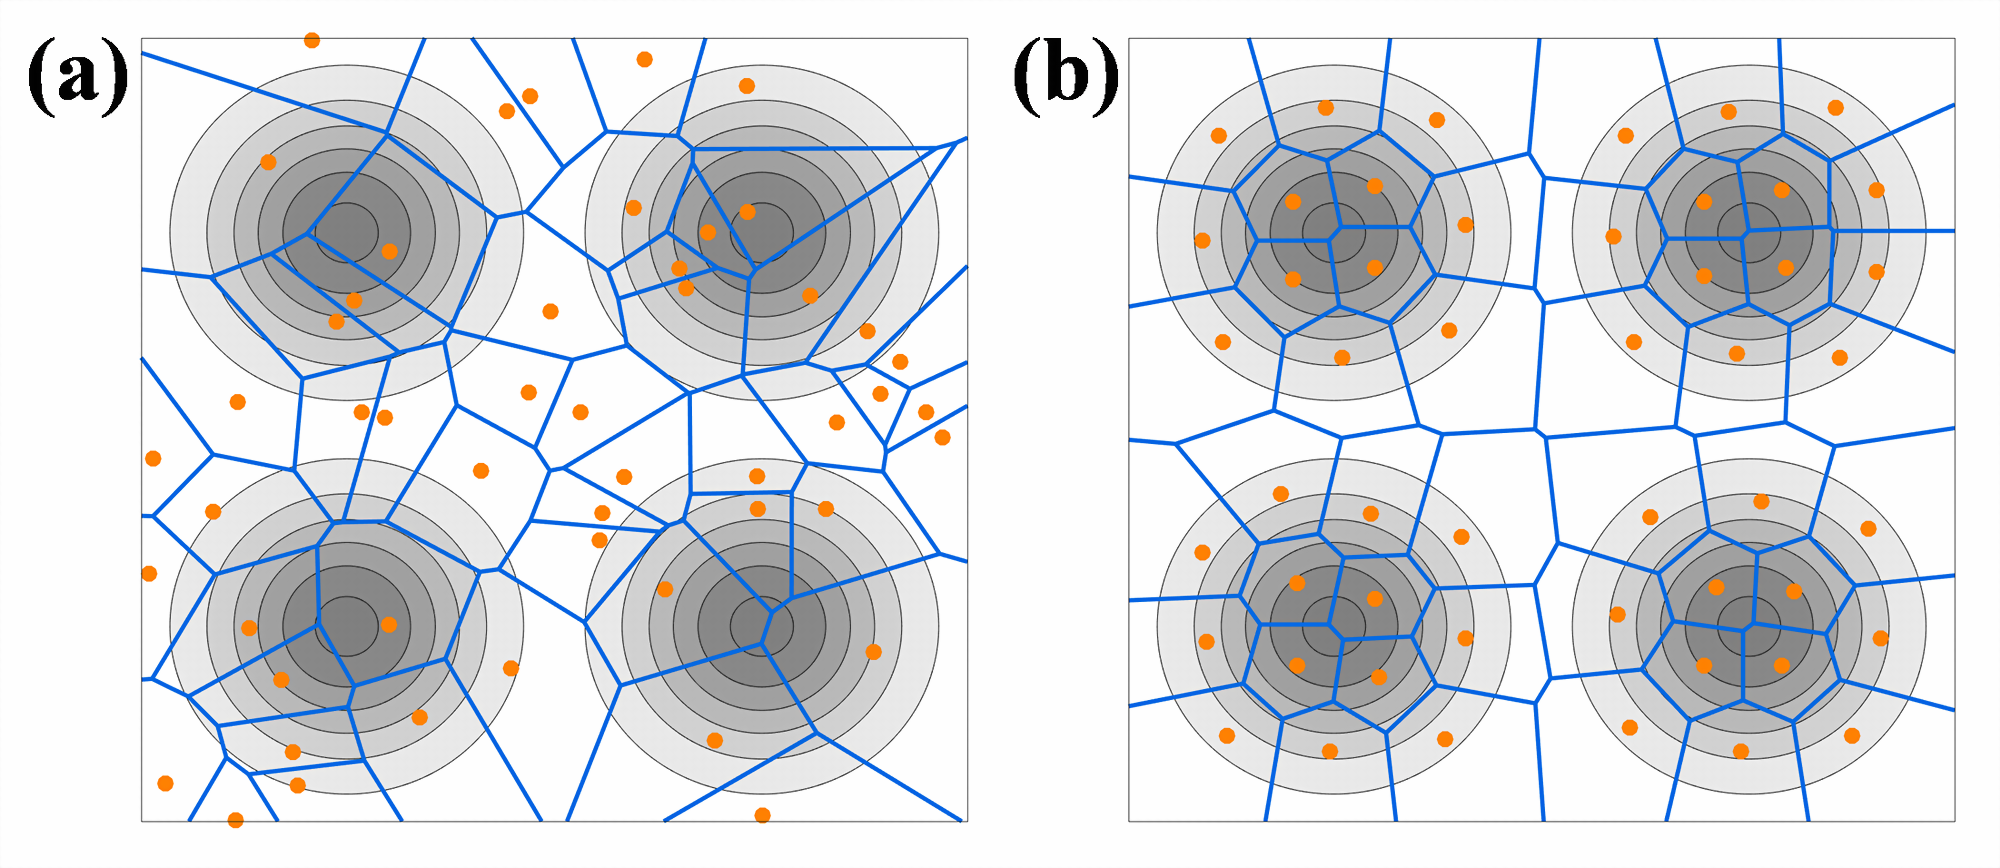
\includegraphics[width=\textwidth]{./cvt/pics/CVT.pdf}
  \end{center}
  \caption{Schematic illustration of the CVT procedure in a 2D domain, including
  (a) initial random choice of centroids and Voronoi tessellation and centroidal
  Voronoi tessellation generated by the weighted K-Means algorithm. The weight
  function is given by  the linear superposition of 4 Gaussian functions.}
  \label{fig:CVT}
\end{figure}

We also show how the interpolation points are placed and moved in real chemical
systems, i.e., the ammonia\hyp{}borane (BH$_3$NH$_3$) decomposition reaction
process. \cref{fig:BH3NH3} (a) shows the electron density of the molecule
at the compressed, equilibrium, and dissociated configurations, respectively,
according to the energy landscape in \cref{fig:BH3NH3} (c). We plot the
interpolation points found by the weighted K\hyp{}Means algorithm in 
\cref{fig:BH3NH3} (b). At the compressed configuration, all the interpolation
points are distributed evenly around the molecule. As the bond length increases,
some interpolation points are transferred from BH$_3$ to NH$_3$. Finally at the
dissociated configuration, NH$_3$ has more interpolation points around the
molecule, since there are more electrons in NH$_3$ than BH$_3$. Along the
decomposition reaction process, both the transfer of the interpolation points
and the potential energy landscape are smooth with respect to the change of the
bond length.

\begin{figure}[htbp]
  \begin{center}
    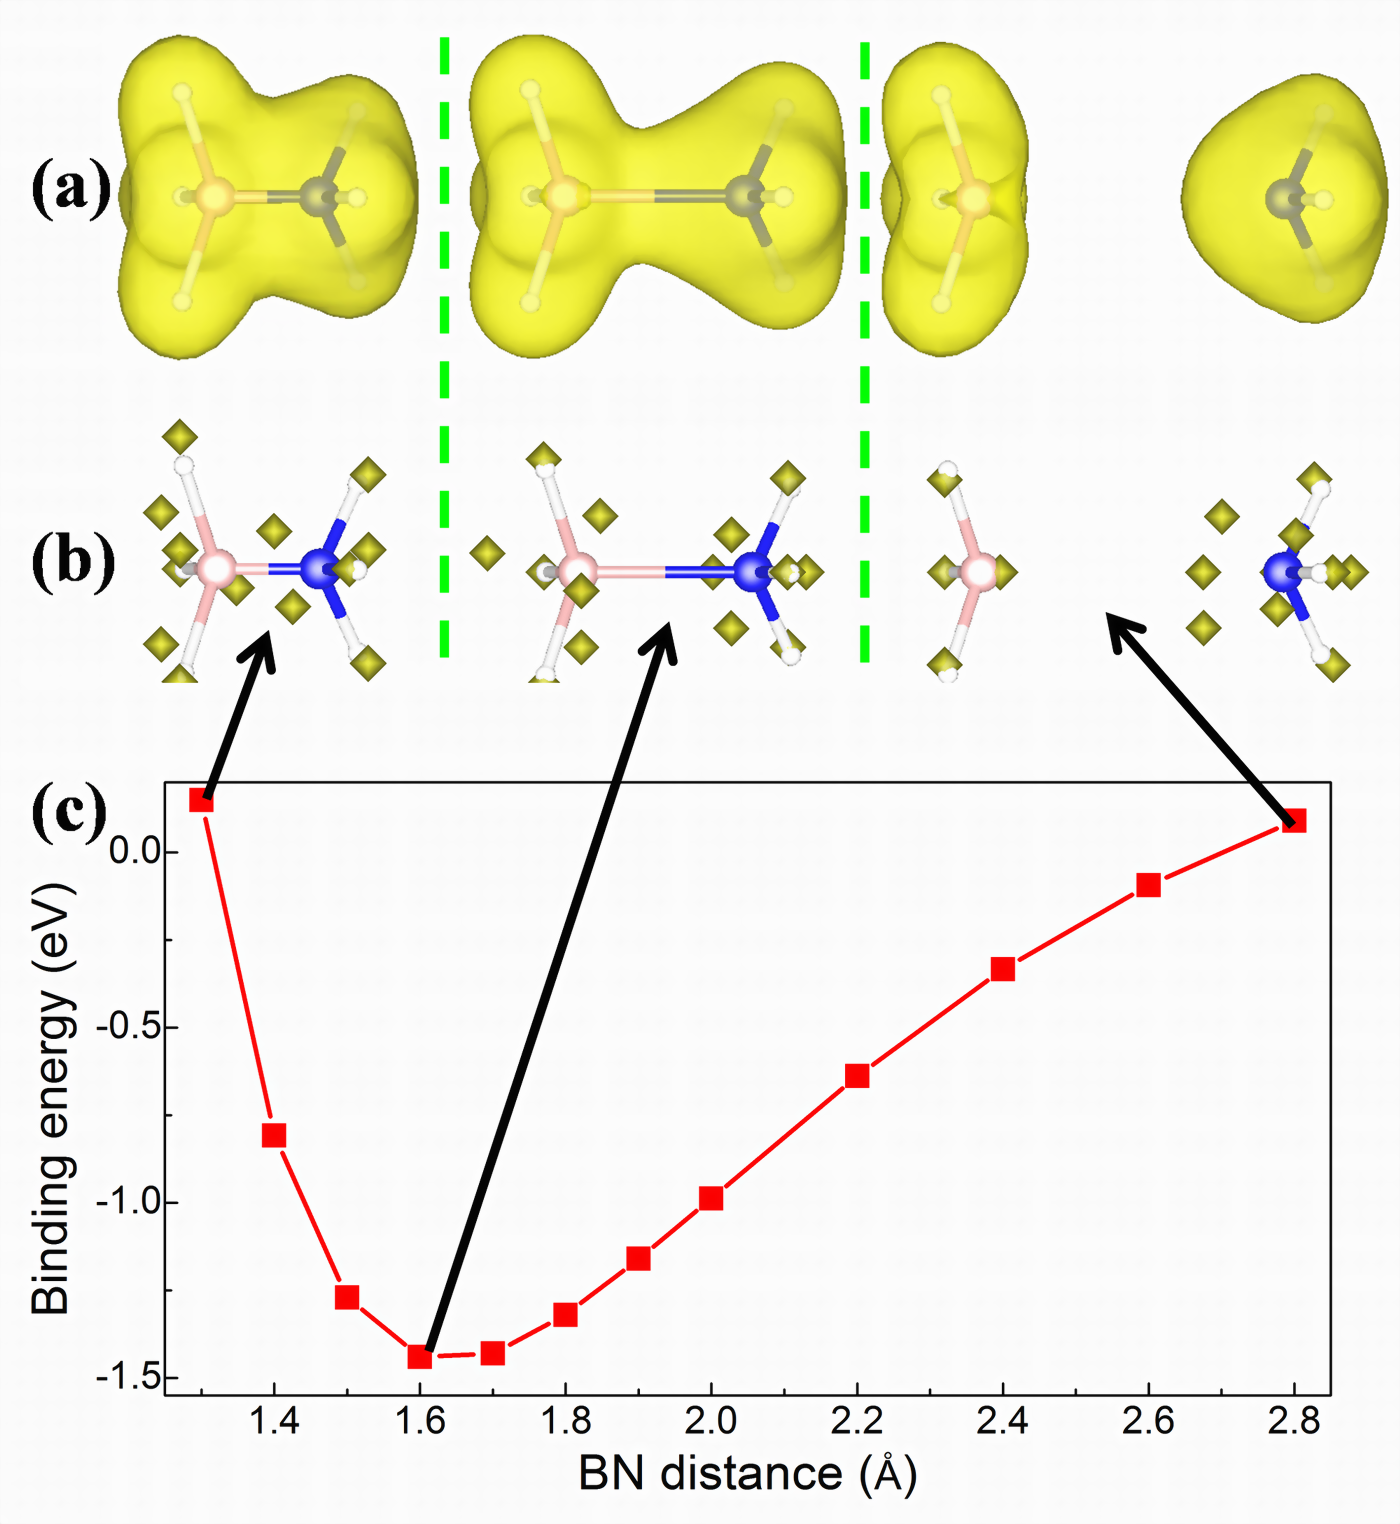
\includegraphics[width=\textwidth]{./cvt/pics/BH3NH3.pdf}
  \end{center}
  \caption{The decomposition reaction process of BH$_3$NH$_3$ computed with
  hybrid functional (HSE06) calculations by using the CVT procedure to select
  interpolation points, including (a) the electron density (yellow isosurfaces),
  (b) the interpolation points (yellow squares) $\{\Brhat_\mu\}_{\mu=1}^{N_
  {\mu}}$ ($N_{\mu}$ = 8) selected from the real space grid points $\{\Br_{i}\}_
  {i=1}^{N_{g}}$ ($N_{g}$ = 100$^3$ and $E_{\text{cut}}$ = 60 Ha) when the BN
  distance respectively is 1.3, 1.7 and 2.8 {\AA} and (c) the binding energy as
  a function of BN distance for BH$_3$NH$_3$ in a 10 {\AA} $\times$ 10 {\AA}
  $\times$ 10 {\AA} box. The white, pink and blue pink balls denote hydrogen,
  boron and nitrogen atoms, respectively.}
  \label{fig:BH3NH3}
\end{figure}